\section{Instruction Set}

The processor implements all required instructions, as shown below:

\begin{itemize}
    \item Several ALU instructions (All working on two registers and storing the result in a third):
        \begin{itemize}
            \item ADD - Addition
            \item SUB - Subtraction
            \item SLT - Test if the first source register is less than second
            \item AND - Bitwise and
            \item OR  - Logical or
        \end{itemize}
    \item BEQ - branch if registers are equal
    \item LW - Load word from memory
    \item SW - Store word to memory
    \item LUI - Store immediate value shifted left 16 bits in a register
    \item J - Jump
\end{itemize}

\section{Architecture}

\begin{figure}[ht]
    \centering
    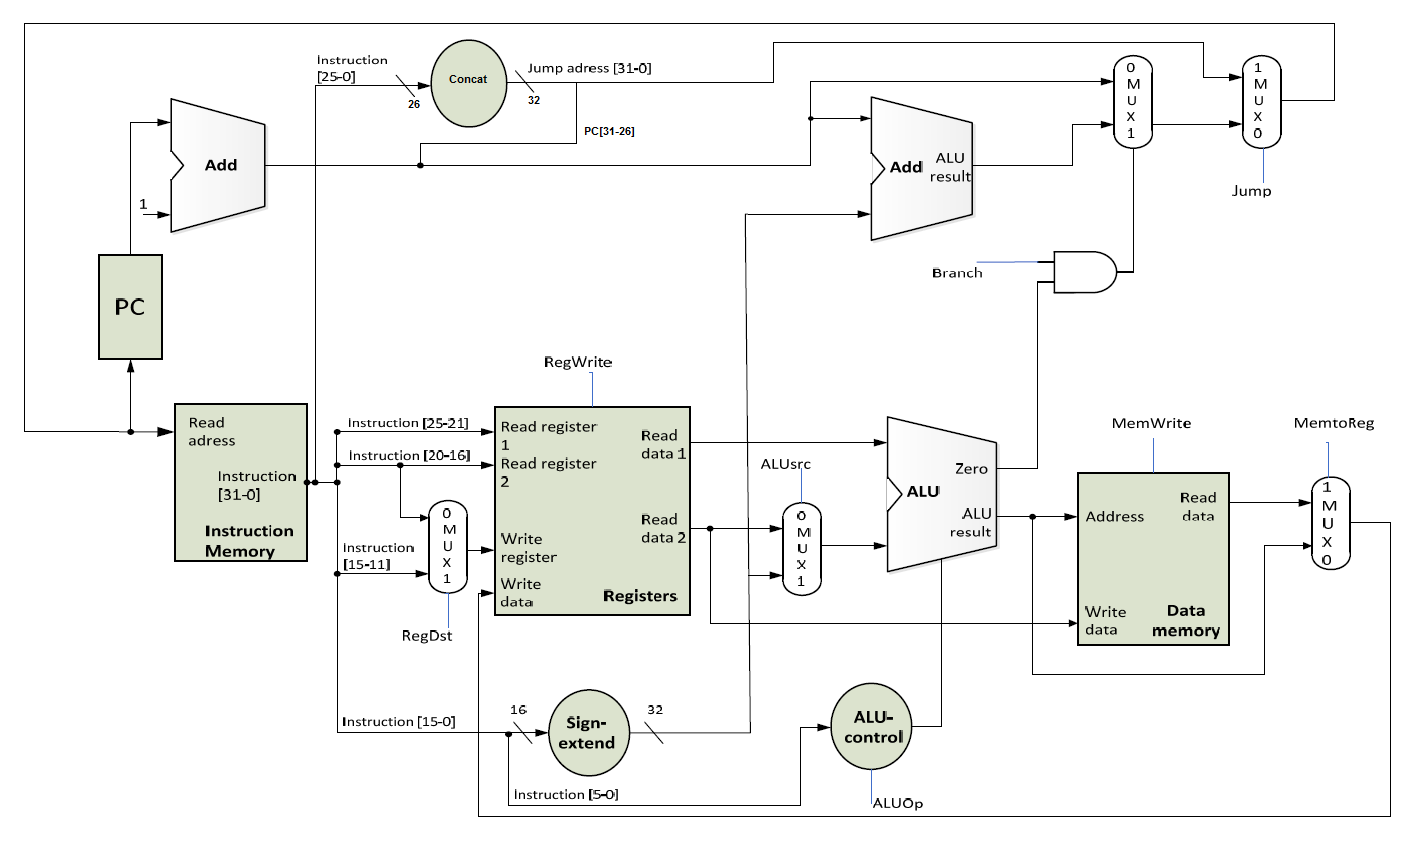
\includegraphics[scale=0.3]{figures/cpu.png}
    \caption{\label{fig:cpuArchitecture}The implemented CPU architecture.} 
\end{figure}

The CPU architecture closely resembles the suggested one.
The main difference is that instead of feeding the program counter register into the instruction memory, %TODO: reference, page 115 compendium
the next calculated program counter is fed into it, and then a flip-flop lets the instruction through at the correct time.

\subsection{The Control Unit}
\begin{figure}[ht]
    \centering
    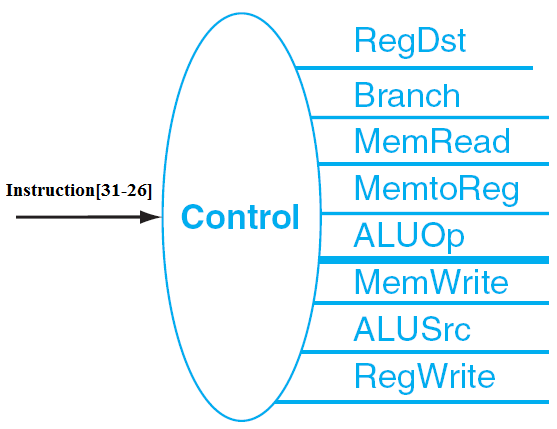
\includegraphics[scale=0.3]{figures/controlunit.png}
    \caption{\label{fig:controlUnit}The control unit.}
\end{figure}

The control unit (CU) was implemented as a state machine, a decoder and a splitter.
On a rising clock edge, it will update the state depending on the current
state. The states, as shown in \ref{fig:stateMachine}, are as follows:

\subsubsection{Fetch}

The instruction is fetched from the instruction memory
and the program counter is updated before the state is set to execute.

\subsubsection{Execute}

The CU lets the ALU and other logic do its things before setting the state to that
decided by the decoder, which is normally fetch, but stall in case of load instructions.

\subsubsection{Stall}

The CU gives the memory an extra cycle to write the data back to the registers, before setting the state to fetch.

\subsubsection{Other}

If the CU finds itself in some other state, something weird has gone wrong.
This is only a sanity check, and should never happen.

\begin{figure}[ht]
    \centering
    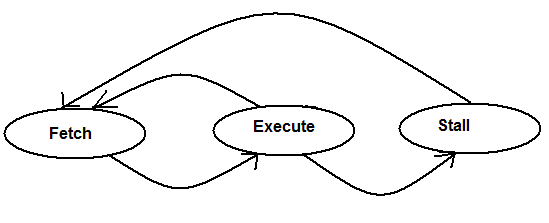
\includegraphics[scale=0.5]{figures/controlunitstatemachine.png}
    \caption{\label{fig:stateMachine}The state machine}
\end{figure}

\subsection{Splitter And Decoder}

The splitter simply splits the signal from the instruction memory into
its induvidual components like opcode, rs, rt, rd and so forth.
The decoder analyzes the opcode and function signals
and enables the correct control signals and decides the next state.
It is composed of a switch statement with one condition-block for each opcode.
The R-format has an additional switch statement to decide the ALU function input.

